\apendice{Documentación de usuario}

\section{Introducción}
En este anexo mostramos en que sistemas se puede usar la aplicación y bajo qué condiciones de manera que la puedan usar los clientes.

\section{Requisitos de usuarios}
El único requisito que necesita un usuario que quiera usar nuestro sistema es un navegador. Necesitamos \eng{javascript} y \eng{cookies} activados, las \eng{cookies} son para mantener la sesión.

Navegadores con los que se ha comprobado:
\begin{enumerate}
\item Firefox 53 
\item Chrome 57
\end{enumerate}


\section{Instalación}
Al proporcionar nuestro servicio como una página web no necesitamos que el cliente o usuario instale la aplicación. 

Si de todas las maneras se hubiese decidido que cada usuario tiene la aplicación en su ordenador se pueden seguir las siguientes instrucciones.


\begin{enumerate}
\setlength{\itemsep}{1pt}
\setlength{\parskip}{0pt}
\setlength{\parsep}{0pt}
\item Se debe comprobar que el ordenador permita la virtualización.
\item Instalar un navegador.
\item Instalar \hfoot{https://docs.docker.com/engine/installation/}{Docker CE}
\item Descargar este archivo \hfoot{https://raw.githubusercontent.com/Jazriel/TFG/master/docker-compose-hub/docker-compose.yml}{Docker compose}.
\item Ejecutar el siguiente comando en un lugar con acceso a internet.

\lstset{style=linestyle}
\begin{lstlisting}[language=bash]
    $ docker-compose pull 
\end{lstlisting}

\item Levantar el servicio con el comando posterior cuando queramos ejecutarlo.

\lstset{style=linestyle}
\begin{lstlisting}[language=bash]
    $ docker-compose up
\end{lstlisting}

\end{enumerate}

Si ejecutamos el 6 con internet se ejecutan tanto el 5 como el 6 ahorrando un mínimo de trabajo.

Cabe destacar que esta instalación es igual para windows y para linux.
 
[captura linux y captura powershell]


\section{Manual del usuario}
El manual de usuario es más simple que otras aplicaciones, esto se debe a que el enfoque del proyecto no ha sido tanto a tener una aplicación con muchas funcionalidades sino a cómo hacerla.

El usuario generalmente llegará a la aplicación por su índice o portada. A esta página generalmente se accede con la dirección IP 127.0.0.1 si la ejecución es local.


\begin{figure}
	\centering
	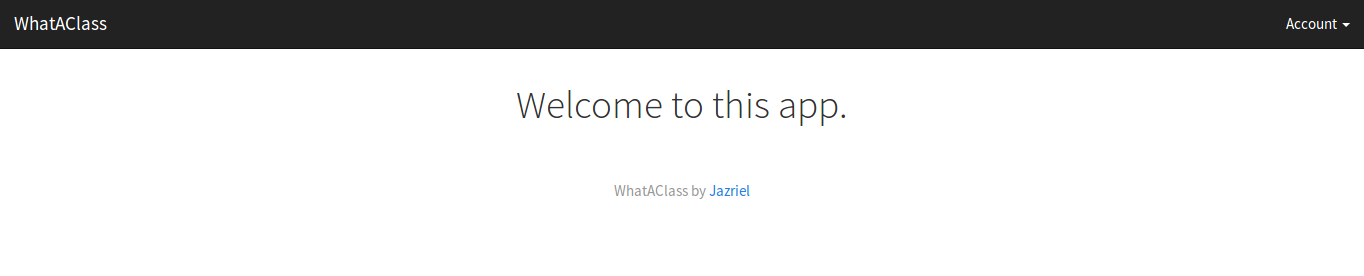
\includegraphics[width=0.8\textwidth]{index.png}
	\caption{Punto de entrada a la aplicación}\label{fig:index.png}
\end{figure}

Para usar la aplicación a partir de ese punto necesita registrarse o iniciar sesión con una de las opciones de inicio de sesión alternativas.

\begin{figure}
	\centering
	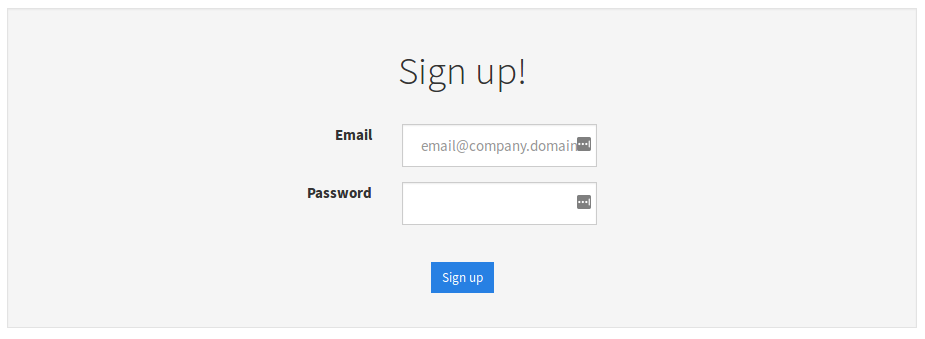
\includegraphics[width=0.8\textwidth]{signup.png}
	\caption{Pantalla de registro de usuario}\label{fig:signup.png}
\end{figure}

Tras registrarse como usuario o tripulante, si esta preparado el correo, se envía un correo electrónico a su dirección personal.

\begin{figure}
	\centering
	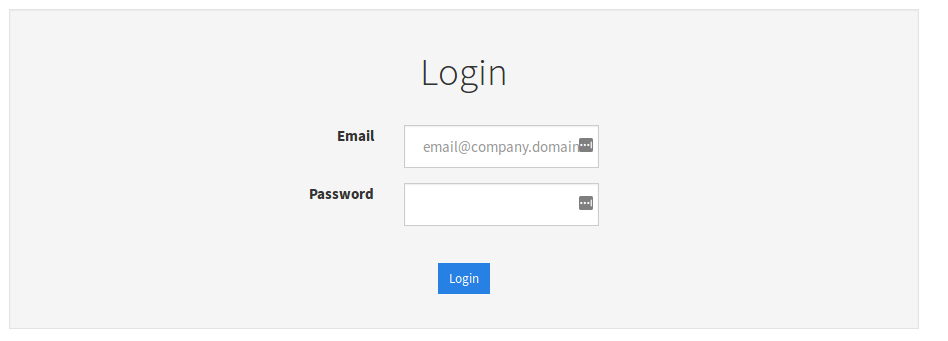
\includegraphics[width=0.8\textwidth]{login.png}
	\caption{Pantalla de inicio de sesión}\label{fig:login.png}
\end{figure}

Una vez se confirma la recepción del correo, se activa la cuenta, permitiendo así usar servicios que antes no estaban disponibles.

\begin{figure}
	\centering
	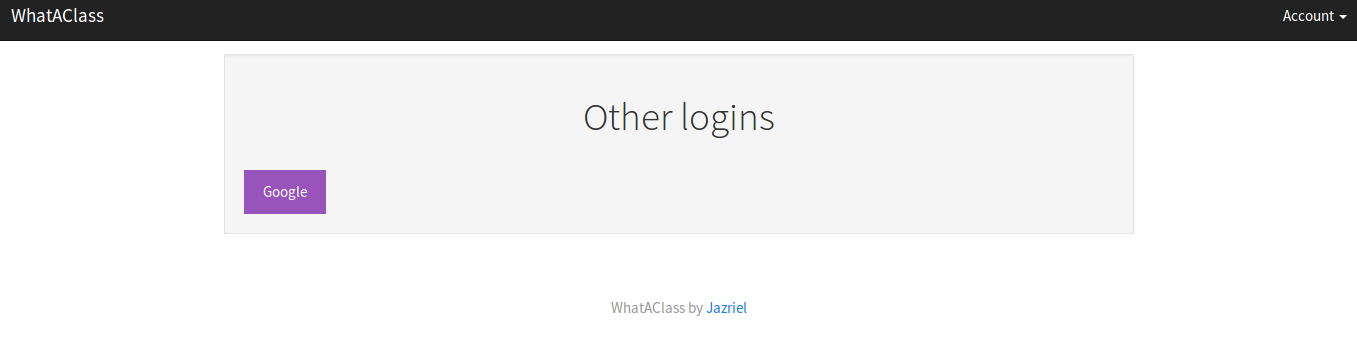
\includegraphics[width=0.8\textwidth]{other_logins.png}
	\caption{Inicios de sesión alternativos}\label{fig:other_logins.png}
\end{figure}


\begin{figure}
	\centering
	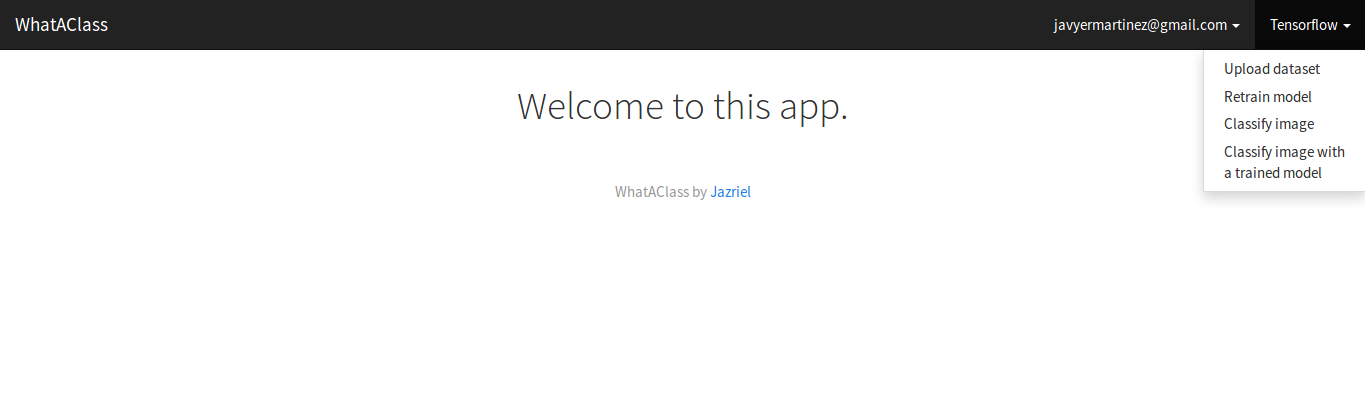
\includegraphics[width=0.8\textwidth]{loggedin.png}
	\caption{Cambio de las zonas accesibles al iniciar sesión}\label{fig:loggedin.png}
\end{figure}


\begin{figure}
	\centering
	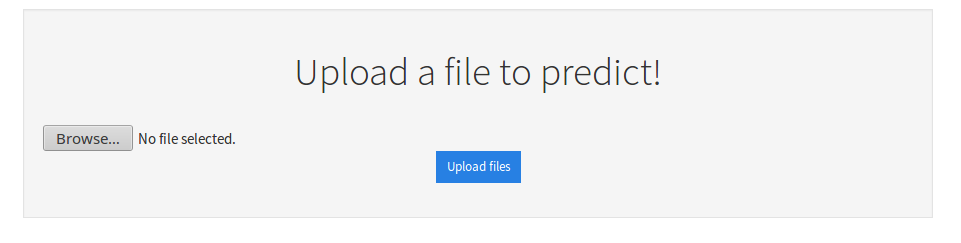
\includegraphics[width=0.8\textwidth]{predict.png}
	\caption{Pantalla de acceso al servicio de clasificación}\label{fig:predict.png}
\end{figure}






